%%%%%%%%%%%%%%%%%%%%%%%%%%%%%%%%%%%%%%%%%%%%%%%%%%%%%%%%%%%%%%%%%%%%%%%%
% CAP�TULO 2
\chapter{CONTROLE MODERNO (xx/xx/2017)}\label{chapter:cap2}

\section{Controle cl�ssico e moderno}

Aqui voc� deve escrever umas 15 linhas ou mais sobre a diferen�a entre controles cl�ssicos e controle moderno. Termine citando os controladores por modos deslizantes e o preditivo.

\section{Controle por modos deslizantes}

Aqui voc� deve falar do controle por modos deslizantes.

\subsection{Sintonia do controlador por modos deslizantes}

Aqui voc� deve dar �nfase nas vari�veis manipuladas do controle por modos deslizantes.

\section{Controle preditivo baseado em modelos}

Aqui voc� deve falar do controle preditivo baseado em modelos.

\subsection{Sintonia do controlador preditivo baseado em modelos}

Aqui voc� deve dar �nfase nas vari�veis manipuladas do controle preditivo baseado em modelos.

\section{Considera��es}

Veja as Figura~\ref{Exep1} e Figura~\ref{Exep2}, que servem de exemplo para inser��o figuras.

\begin{figure}[!h]
	\centering
	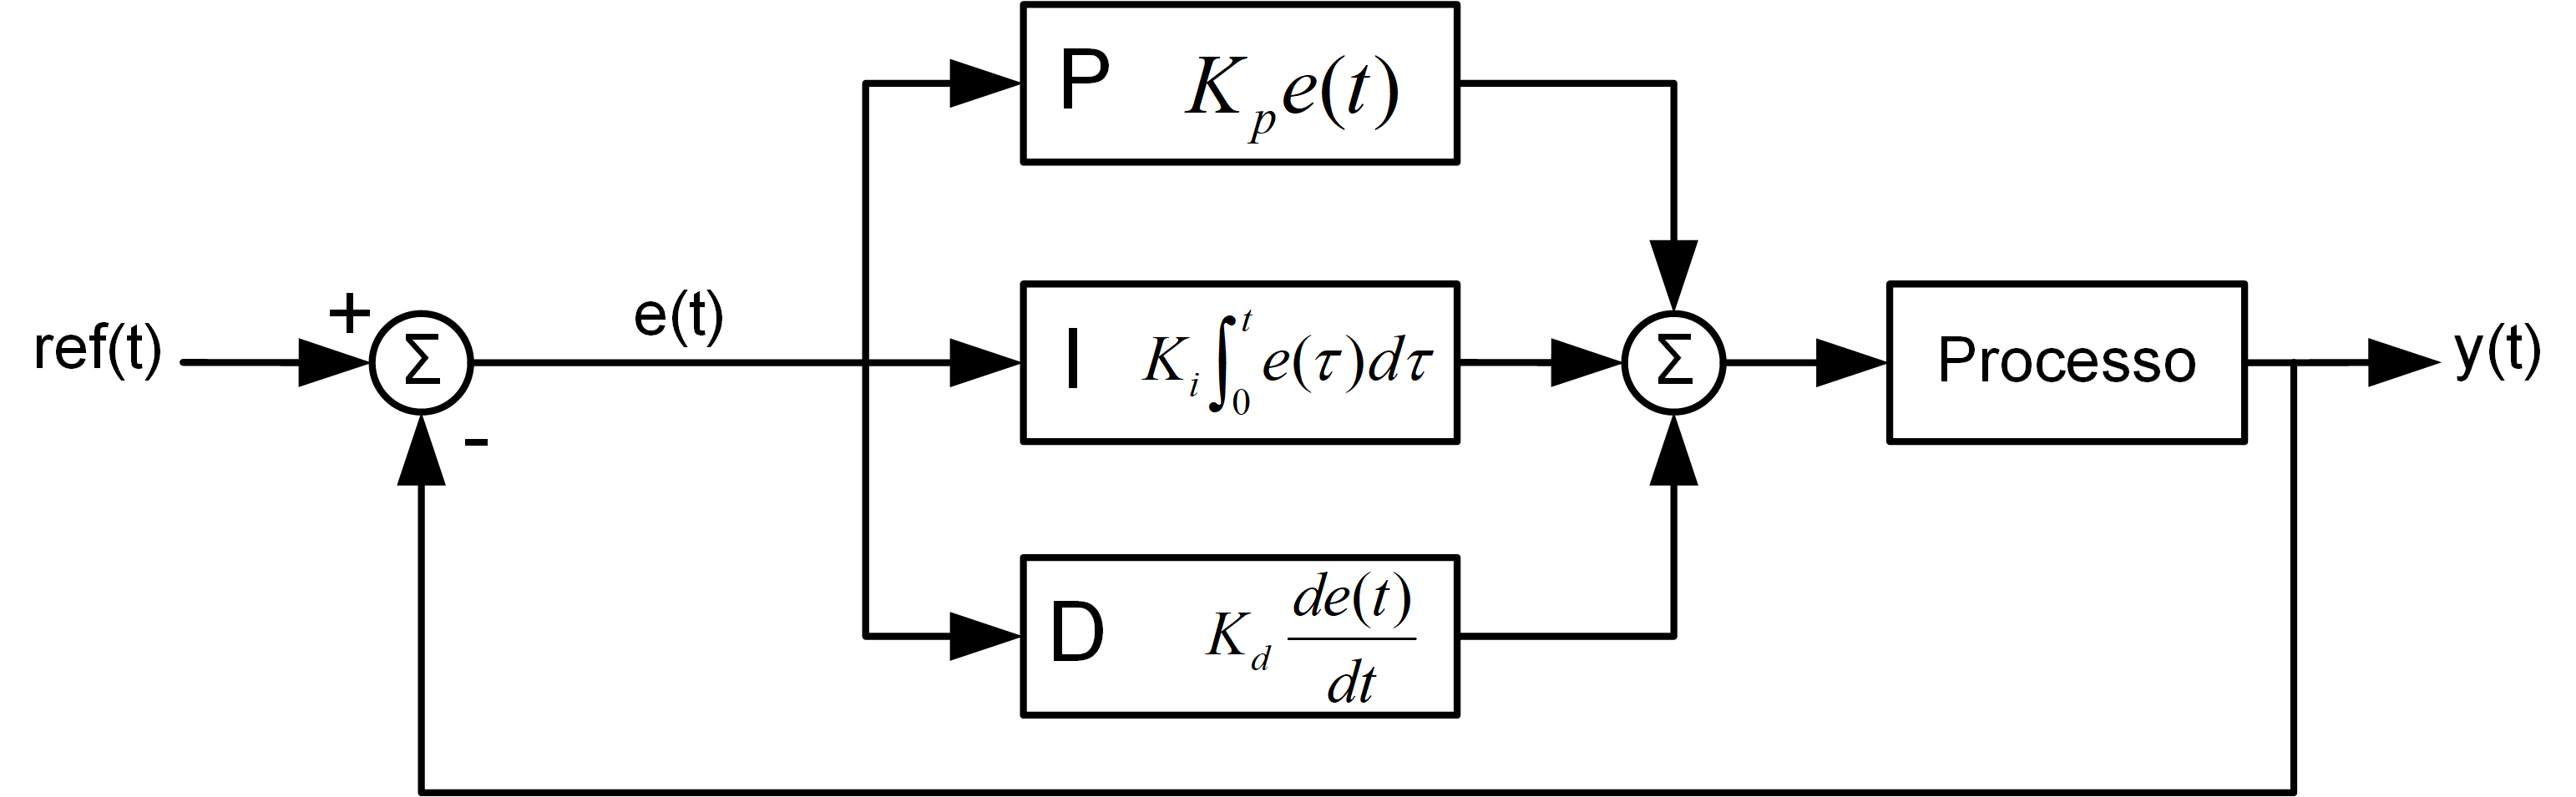
\includegraphics[width=20pc]{./figs/Fig1-1}
	\caption{Partes construtivas do motor de corrente cont�nua.}
	\label{Exep1}
\end{figure} 

\begin{figure}[!h]
	\begin{center}
		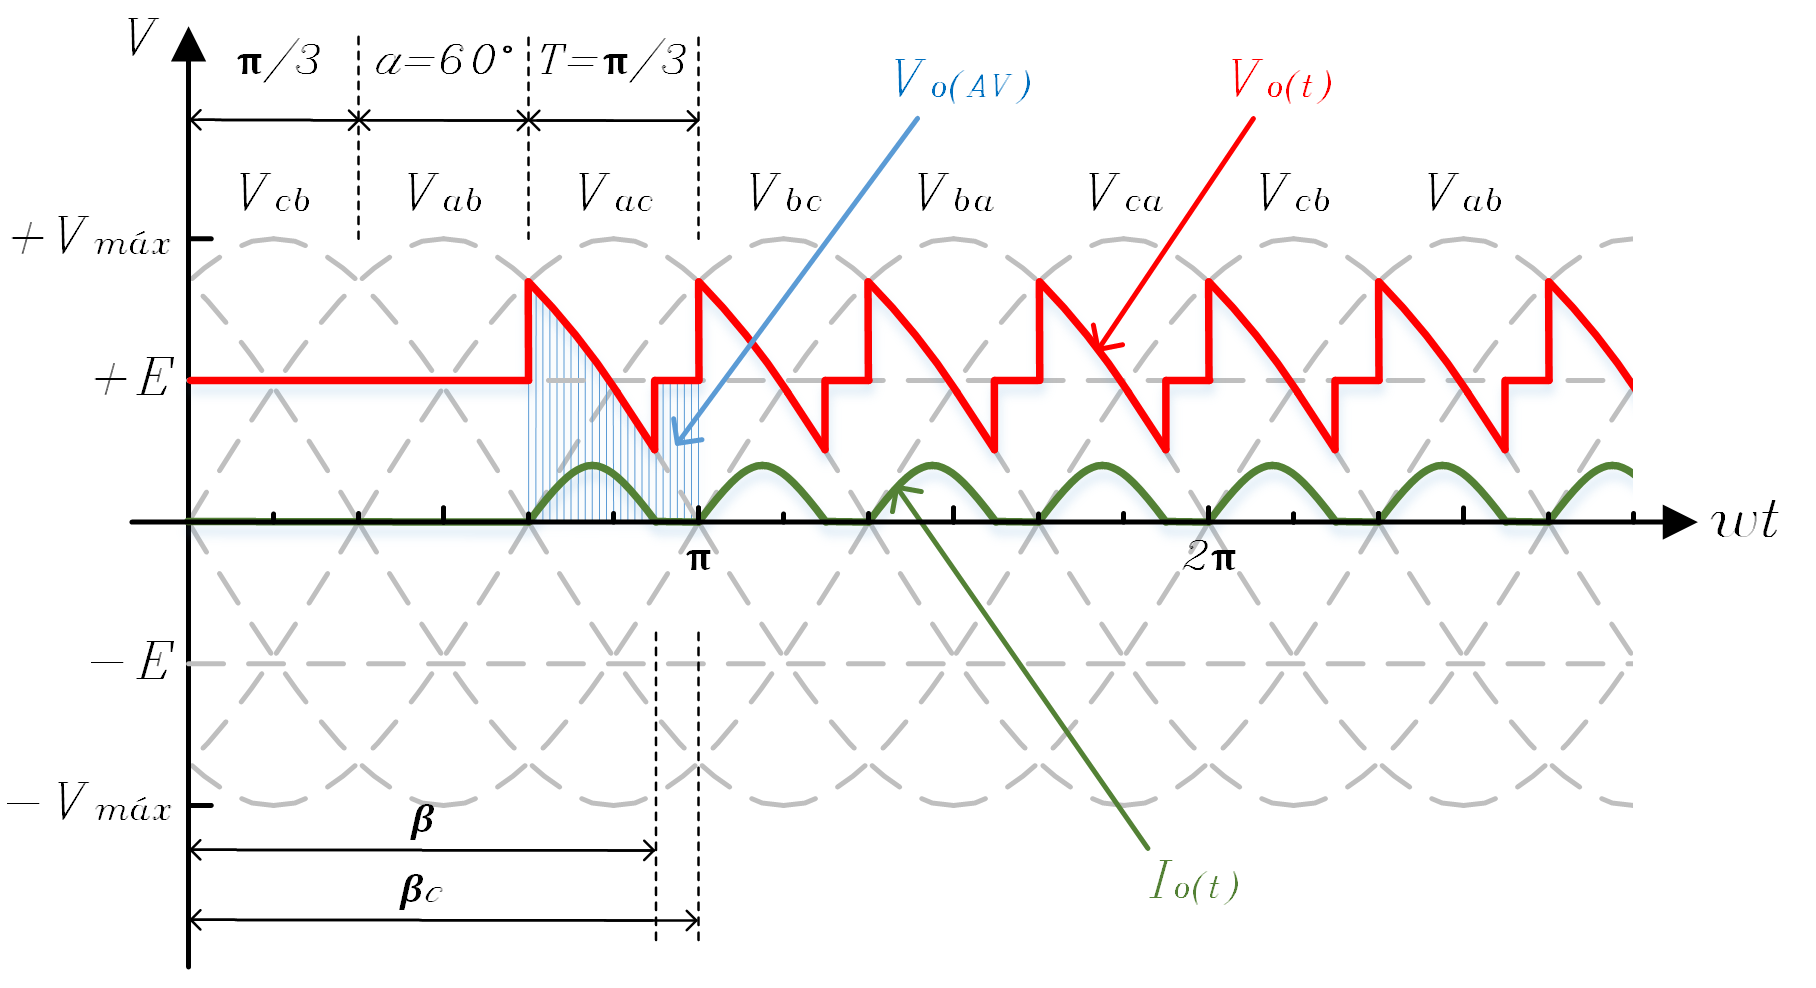
\includegraphics[width=\linewidth]{./figs/Fig2-4}
		\caption{Liga��es de m�quinas CC: (a) excita��o independente, (b) em deriva��o, (c) em s�rie, (d) composta.}
		\label{Exep2}
	\end{center}
\end{figure}